\section{Техническое задание}
\subsection{Основание для разработки}

Полное наименование системы: «Программно-информационная система для создания и работы с аудиозаписями. Подсистема анализа и улучшения качества». Основанием для разработки программы является приказ ректора ЮЗГУ от «17» апреля 2025 г. №1828-с «Об утверждении тем выпускных квалификационных работ».

\subsection{Цель и назначение разработки}

Создание удобного и функционального инструмента для обработки аудиофайлов с возможностью применения различных звуковых эффектов в реальном времени, визуализации аудиоданных и сохранения результатов обработки. Назначение программы - предоставить пользователям простой в использовании, но мощный инструмент для базовой звуковой обработки, включающий эквалайзер, компрессор и ревербератор, с интуитивно понятным графическим интерфейсом и визуальной обратной связью. Код реализует многопоточную обработку аудио для минимизации задержек, поддерживает загрузку различных аудиоформатов, обеспечивает плавную визуализацию формы волны и частотного спектра, а также предлагает оптимизированные алгоритмы обработки звука. Приложение предназначено для музыкантов, звукорежиссеров и людей, которым требуется быстрый доступ к основным инструментам звуковой обработки без необходимости использования сложных профессиональных DAW.

\subsection{Требования к программной системе}

\subsubsection{Требования к данным программной системы}

Входные данные:
\begin{itemize}
	\item аудиофайлы форматов WAV, MP3, OGG, FLAC;
	\item параметры эффектов (эквалайзер, компрессор, реверберация), задаваемые пользователем.
\end{itemize}

Обрабатываемые данные:
\begin{itemize}
	\item аудиосигнал в виде массива numpy.ndarray (форма (N, 1) для моно, (N, 2) для стерео); 
	\item частота дискретизации (стандартно 44100 Гц, но поддерживаются другие значения);
	\item временные и спектральные данные для визуализации (форма волны, частотный спектр).
\end{itemize}

Выходные данные:
\begin{itemize}
	\item обработанный аудиофайл (экспорт в WAV, MP3);
	\item графики формы сигнала и АЧХ в реальном времени.
\end{itemize}

\subsubsection{Функциональные требования к программной системе}

В разрабатываемой программе пользователь может:
\begin{itemize}
	\item загружать аудиофайлы разных форматов (wav, mp3, ogg, flac);
	\item экспортировать результат, с применением выбранных им эффектов, в двух форматах: wav и mp3;
	\item воспроизводить, останавливать аудио, изменить позицию воспроизведения, узнать текущее время проигрывания;
	\item применять эффекты в режиме реального времени, включать и отключать их;
	\item применить эквалайзер, настроить низкие/средние/высокие частоты;
	\item применить компрессор, настроить порог, коэффициент сжатия, время атаки и восстановления сигнала, усиление;
	\item применить реверберацию, настроить уровень эффекта, размер комнаты, затухание и чистый звук;
	\item видеть форму сигнала в режиме реального времени, посмотреть АЧХ аудио.
\end{itemize}

На рисунке \ref{fig:use_case_diagram} изображена диаграмма прецедентов

\begin{figure}[ht]
	\center{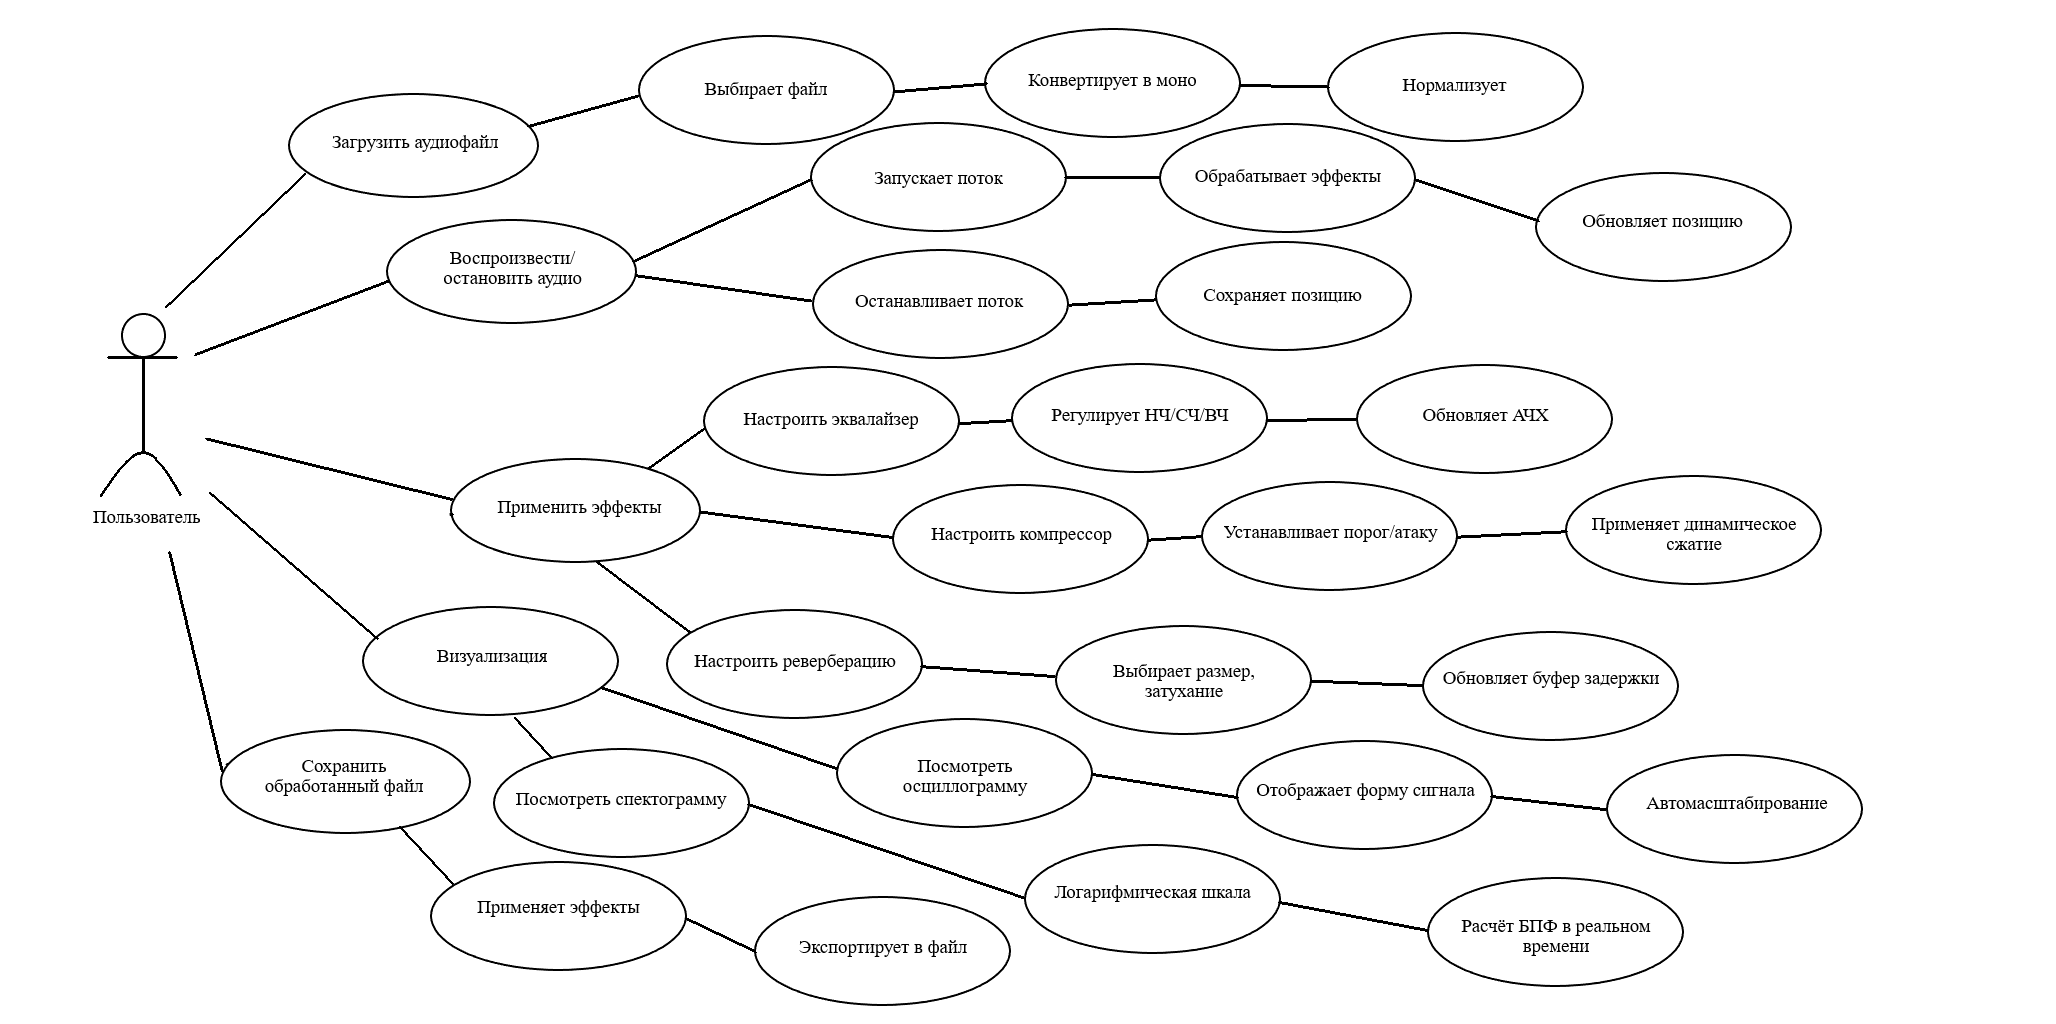
\includegraphics[width=1\linewidth]{DiagramPrec}}
	\caption{Диаграмма прецедентов}
	\label{fig:use_case_diagram}
\end{figure}

\paragraph{Вариант использования «Оформление заказа»}
Заинтересованные лица и их требования: пользователь хочет загрузить аудиофайл для последующей обработки.

Требования: поддержка форматов (WAV, MP3, OGG, FLAC), автоматическая конвертация в моно, нормализация амплитуды.

Предусловие: приложение запущено, файл существует и доступен для чтения.

Постусловие: аудиоданные загружены в память, форма волны отображена на графике, кнопки "Воспроизвести" и "Сохранить" активированы.

Основной успешный сценарий:
\begin{enumerate}
	\item Пользователь нажимает кнопку "Загрузить".
	\item Открывается диалоговое окно выбора файла.
	\item Пользователь выбирает файл и подтверждает выбор.
\end{enumerate}

\paragraph{Вариант использования «Воспроизведение аудио»}

Заинтересованные лица и их требования: пользователь хочет прослушать загруженный файл с возможностью применения эффектов в реальном времени.

Предусловие: аудиофайл успешно загружен, аудиоустройство вывода доступно.

Постусловие: аудиопоток запущен, графики обновляются в реальном времени.

Основной успешный сценарий:
\begin{enumerate}
	\item Пользователь нажимает кнопку «Воспроизвести».
	\item Система инициализирует аудиопоток
	\item Callback-функция начинает передавать данные в устройство.
	\item Позиция воспроизведения обновляется каждые 100 мс.
	\item Сигнал и АЧХ отображаются в реальном времени.
\end{enumerate}

\paragraph{Вариант использования «Остановка воспроизведения»}

Заинтересованные лица и их требования: пользователь хочет немедленно прекратить воспроизведение аудио.

Предусловие: идёт воспроизведение аудиофайла.

Постусловие: аудиопоток полностью остановлен, интерфейс обновлен.

Основной успешный сценарий:
\begin{enumerate}
	\item Пользователь нажимает кнопку "Стоп".
	\item Система останавливает воспроизведение аудио.
	\item Текущая позиция фиксируется для возможности дальнейшего продолжения.
\end{enumerate}

\paragraph{Вариант использования «Изменения позиции воспроизведения»}

Заинтересованные лица и их требования: пользователь хочет перемотать аудио на произвольную позицию.

Предусловие: аудиофайл загружен.

Постусловие: текущая позиция воспроизведения изменена, при активном воспроизведении звук продолжается с новой позиции, интерфейс синхронизирован.

Основной успешный сценарий:
\begin{enumerate}
	\item Пользователь перемещает ползунок позиции мышью.
	\item Система пересчитывает позицию.
	\item При воспроизведении поток начинает чтение с новой позиции.
\end{enumerate}

\paragraph{Вариант использования «Применения эквалайзера»}

Заинтересованные лица и их требования: пользователь хочет настроить частотный баланс (НЧ/СЧ/ВЧ).

Предусловие: файл загружен, вкладка "Эквалайзер" открыта.

Постусловие: параметры эквалайзера применены к аудиопотоку, график АЧХ обновлен.

Основной успешный сценарий:
\begin{enumerate}
	\item Пользователь включает чекбокс «Эквалайзер».
	\item Регулирует ползунки НЧ/СЧ/ВЧ.
	\item Система пересчитывает коэффициент БИХ-фильтров.
	\item Аудиозапись изменяется в соответствии с настройками пользователя.
	\item АЧХ отображается на графике.
\end{enumerate}

\paragraph{Вариант использования «Применения компрессора»}

Заинтересованные лица и их требования: пользователь хочет изменить динамический диапазон аудиосигнала для более равномерного звучания.

Предусловие: аудиофайл успешно загружен, вкладка "Компрессор" открыта.

Постусловие: параметры компрессора применены к аудиопотоку, изменения слышны при воспроизведении.

Основной успешный сценарий:
\begin{enumerate}
	\item Пользователь активирует чекбокс «Компрессор».
	\item Устанавливает порог, коэффициент компрессии, время атаки и восстановления, усиление выходного сигнала.
	\item Аудио обрабатывается в режиме реального времени.
\end{enumerate}

\paragraph{Вариант использования «Применения реверберации»}

Заинтересованные лица и их требования: пользователь хочет добавить эффект реверберации к аудиосигналу.

Предусловие: аудиофайл успешно загружен, вкладка "Реверберация" открыта.

Постусловие: эффект реверберации применен к аудиопотоку, буфер реверберации инициализирован с новыми параметрами.

Основной успешный сценарий:
\begin{enumerate}
	\item Пользователь активирует чекбокс "Реверберация".
	\item Пользователь регулирует параметры: уровень эффекта, исходный звук, размер комнаты, затухание.
	\item Аудио обрабатывается в режиме реального времени.
\end{enumerate}	

\paragraph{Вариант использования «Сохранение обработанного файла»}

Заинтересованные лица и их требования: пользователь хочет экспортировать результат с примененными эффектами.

Предусловие: файл загружен, эффекты настроены.

Постусловие: файл сохранен на диск в выбранном формате.

Основной успешный сценарий:
\begin{enumerate}
	\item Пользователь нажимает "Сохранить".
	\item Открывается диалог выбора формата (WAV/MP3) и пути.
	\item Пользователь выбирает формат, путь и название файла.
	\item Система применяет выбранные эффекты, экспортирует файл.
	\item Файл успешно сохранён на диске.
\end{enumerate}		

\paragraph{Вариант использования «Визуализация данных»}

Заинтересованные лица и их требования: пользователь хочет видеть графическое представление аудиосигнала.

Предусловие: аудиофайл загружен и идет воспроизведение.

Постусловие: графики формы волны и АЧХ отображаются и обновляются в режиме реального времени.

Основной успешный сценарий:
\begin{enumerate}
	\item Пользователь нажимает «Воспроизвести».
	\item Система отображает графики формы волны и АЧХ.
\end{enumerate}	

%-------------------------------------------------------------------------------
\subsubsection{Требования пользователя к интерфейсу веб-приложения}

Приложение должно иметь следующие основные функции:
\begin{enumerate}
	\item Основные элементы управления - кнопки управления воспроизведением: "Загрузить", "Воспроизвести", "Стоп", "Сохранить". Ползунок позиции воспроизведения, точное позиционирование, индикатор текущей позиции в формате MM:SS / MM:SS.
	\item Визуализация аудио - два синхронизированных графика: верхний график формы волны и нижний график амплитудно-частотной характеристики. Подписи осей с единицами измерения (амплитуда, частота).
	\item Панель эффектов (вкладки):
	\begin{enumerate}
		\item Эквалайзер - Три ползунка с подписями: низкие частоты (150Hz): ±24 дБ, средние частоты (1kHz): ±24 дБ, высокие частоты (5kHz): ±24 дБ. Чекбокс активации эффекта.
		\item Компрессор - ползунки параметров: порог: -60..0 дБ, соотношение: 1..20, атака: 1..500 мс, восстановление: 10..2000 мс, усиление: 0..24 дБ. Чекбокс активации эффекта.
		\item Реверберация: ползунки параметров: уровень эффекта: 0..1, сухой сигнал: 0..1, размер помещения: 0.1..2.0, затухание: 0.1..0.9. Чекбокс активации эффекта.
	\end{enumerate}	
	\item Обратная связь и состояние: индикатор загрузки при обработке файлов. Всплывающие уведомления об ошибках: при неудачной загрузке файла, при проблемах с аудиоустройством, при ошибках сохранения. Изменение состояния кнопок: "Воспроизвести" активна только при загруженном файле, "Стоп" активна только во время воспроизведения, "Сохранить" активна только после загрузки файла.
	\item Производительность: задержка отклика интерфейса не более 100 мс, плавная анимация графиков без рывков, минимальное потребление ресурсов в фоновом режиме.
\end{enumerate}	

\subsubsection{Нефункциональные требования к программной системе}

\paragraph{Требования к надёжности}

В процессе работы аудио-процессора могут возникнуть следующие аварийные ситуации:
\begin{itemize}
	\item потеря доступа к аудиоустройству в связи с его отключением, изменением системных настроек звука или конфликтом с другим приложением;
	\item попытка загрузки повреждённого или неподдерживаемого аудиофайла с несовместимым форматом, битрейтом или частотой дискретизации;
	\item неожиданное прекращение работы из-за нехватки системных ресурсов при обработке объёмных файлов или одновременном применении нескольких ресурсоёмких эффектов;
	\item ошибки в работе эффектов обработки звука, приводящие к искажению аудиосигнала или сбоям в воспроизведении.
\end{itemize}

Приложение должно автоматически определять доступные аудиоустройства и переключаться между ними при потере соединения с текущим устройством. В случае невозможности восстановления подключения система должна сохранять возможность обработки звука без функции воспроизведения с уведомлением пользователя о возникшей проблеме.

Для работы с аудиофайлами приложение должно проверять их целостность и соответствие поддерживаемым форматам перед загрузкой, а также автоматически выполнять необходимые преобразования (нормализацию, конвертацию в моно, приведение к стандартной частоте дискретизации). При обнаружении критических ошибок в файле пользователь должен получить понятное сообщение о проблеме с указанием конкретной причины.

Для предотвращения аварийного завершения из-за нехватки ресурсов система должна контролировать использование оперативной памяти и процессорного времени, ограничивать размеры буферов обработки и корректно завершать работу при приближении к предельным значениям. Все параметры эффектов и текущее состояние обработки должны сохраняться даже при аварийном завершении работы.

При возникновении ошибок в работе эффектов обработки звука система должна автоматически сбрасывать параметры эффектов к безопасным значениям, сохраняя при этом возможность дальнейшей работы. Все критические ошибки должны фиксироваться в системном логе с указанием времени возникновения, типа ошибки и состояния системы на момент сбоя.

\paragraph{Требования к безопасности}

Требования к приложению:
\begin{enumerate}
	\item Перед загрузкой файла, система должна проверять формат и корректность заголовков. При обнаружении повреждённых данных программа будет выводить ошибку без попытки обработки.
	\item Для безопасности управления памятью и ресурсами необходима изоляция обработки аудио, то есть каждый эффект будет применяться в отдельном потоке с контролем потребления ресурсов и будет ограничен буфе. Так же потребуется очистка временных данных, чтобы после завершения обработки или при ошибке все промежуточные буферы будут очищаться.
	\item Для защиты от вирусов применится проверка структуры файлов, анализ сигнатуры файла перед декодированием, ограничение максимальной длительности обрабатываемого аудио.
	\item Пользовательские настройки будут проверятся перед применением, а недопустимые значения автоматически скорректируются до ближайших безопасных.
	\item При завершении работы, приложение будет останавливать все потоки, освобождать аудиоустройства.
\end{enumerate}

\paragraph{Требования к программному обеспечению}

Для реализации программы будет использоваться язык программирования Python и библиотеки: NumPy, SciPy, PyDub, SoundDevice, Matplotlib, Numba.

Для работы приложения требуется Windows 10/11 (64-bit)

\paragraph{Требования к аппаратному обеспечению}

Минимальная конфигурация:

Центральный процессор с количеством ядер от 2 и выше с тактовой частотой от 2.0 ГГц. Поддержка инструкций SSE4.2. Оперативная память - 4 ГБ. 100 МБ свободного места для установки. Поддержка ASIO/WASAPI для профессионального использования.

\subsubsection{Требования к оформлению документации}

Требования к стадиям разработки программ и программной документации для вычислительных машин, комплексов и систем независимо от их назначения и области применения, этапам и содержанию работ устанавливаются ГОСТ 19.102-77
Программная документация должна включать в себя:
\begin{itemize}
	\item анализ предметной области;
	\item техническое задание;
	\item технический проект.
\end{itemize}
